% THIS IS SIGPROC-SP.TEX - VERSION 3.1
% WORKS WITH V3.2SP OF ACM_PROC_ARTICLE-SP.CLS
% APRIL 2009
%
% It is an example file showing how to use the 'acm_proc_article-sp.cls' V3.2SP
% LaTeX2e document class file for Conference Proceedings submissions.
% ----------------------------------------------------------------------------------------------------------------
% This .tex file (and associated .cls V3.2SP) *DOES NOT* produce:
%       1) The Permission Statement
%       2) The Conference (location) Info information
%       3) The Copyright Line with ACM data
%       4) Page numbering
% ---------------------------------------------------------------------------------------------------------------
% It is an example which *does* use the .bib file (from which the .bbl file
% is produced).
% REMEMBER HOWEVER: After having produced the .bbl file,
% and prior to final submission,
% you need to 'insert'  your .bbl file into your source .tex file so as to provide
% ONE 'self-contained' source file.
%
% Questions regarding SIGS should be sent to
% Adrienne Griscti ---> griscti@acm.org
%
% Questions/suggestions regarding the guidelines, .tex and .cls files, etc. to
% Gerald Murray ---> murray@hq.acm.org
%
% For tracking purposes - this is V3.1SP - APRIL 2009

\documentclass{acm_proc_article-sp}

\begin{document}

\title{Non-hierarchical Social Learning via Reward-Based Update Filtering}
%
% You need the command \numberofauthors to handle the 'placement
% and alignment' of the authors beneath the title.
%
% For aesthetic reasons, we recommend 'three authors at a time'
% i.e. three 'name/affiliation blocks' be placed beneath the title.
%
% NOTE: You are NOT restricted in how many 'rows' of
% "name/affiliations" may appear. We just ask that you restrict
% the number of 'columns' to three.
%
% Because of the available 'opening page real-estate'
% we ask you to refrain from putting more than six authors
% (two rows with three columns) beneath the article title.
% More than six makes the first-page appear very cluttered indeed.
%
% Use the \alignauthor commands to handle the names
% and affiliations for an 'aesthetic maximum' of six authors.
% Add names, affiliations, addresses for
% the seventh etc. author(s) as the argument for the
% \additionalauthors command.
% These 'additional authors' will be output/set for you
% without further effort on your part as the last section in
% the body of your article BEFORE References or any Appendices.

\numberofauthors{2} %  in this sample file, there are a *total*
% of EIGHT authors. SIX appear on the 'first-page' (for formatting
% reasons) and the remaining two appear in the \additionalauthors section.
%
\author{
% You can go ahead and credit any number of authors here,
% e.g. one 'row of three' or two rows (consisting of one row of three
% and a second row of one, two or three).
%
% The command \alignauthor (no curly braces needed) should
% precede each author name, affiliation/snail-mail address and
% e-mail address. Additionally, tag each line of
% affiliation/address with \affaddr, and tag the
% e-mail address with \email.
%
% 1st. author
\alignauthor
Wesley Tansey\\
       \affaddr{Dept. of Computer Science, The University of Texas at Austin}\\
       \affaddr{1 University Station C0500, Austin, TX, USA}\\
       \email{tansey@cs.utexas.edu}
\alignauthor
Eli Feasley\\
       \affaddr{Dept. of Computer Science, The University of Texas at Austin}\\
       \affaddr{1 University Station C0500, Austin, TX, USA}\\
       \email{elie@cs.utexas.edu}
}
\date{12 December 2011}
% Just remember to make sure that the TOTAL number of authors
% is the number that will appear on the first page PLUS the
% number that will appear in the \additionalauthors section.

\maketitle
\begin{abstract}
Social learning is an extension to Evolutionary Algorithms that enables individuals to learn from observations of others in the population.
 Traditionally, social learning algorithms have employed a student-teacher model where the behavior of one group of individuals is used to train the remaining individuals in the population.  
 We present a non-hierarchical model of social learning in which we do not label each agent, instead allowing any individual which experiences positive reward to teach the rest of the agents on its recent behavior. 
 We validate our approach in a foraging domain, comparing social learning in both Darwinian and Lamarkian paradigms to a standard Darwinian evolution with no learning. 
 We show that our non-hierarchical form facilitates rapid discovery of near-optimal solutions.  While Lamarkian evolution eventually produces a regression-to-the-mean effect, we bootstrap several generations of Lamarkian evolution with regular GAs to produce a highly efficient solution to the foraging problem.
\end{abstract}

% A category with the (minimum) three required fields
%\category{D.4.6}{Security and Protection}{Authorization}
%A category including the fourth, optional field follows...
%\category{K.6.5}{Security and Protection}{Authorization}
%\category{E.3}{Data Encryption}{Code breaking}

\terms{Social Learning, Evolutionary Algorithms, Artificial Life}

\section{Introduction} 
	In Evolutionary Algorithms, individual agents often learn within a world and then die or reproduce without passing on the knowledge they have learned.  This is wasteful, especially in domains that are difficult or impossible to simulate, like realistic environments or real-life data.  Social learning represents a way to share knowledge without the expense of sending each individual throught the world many times.
	Various animals have brains that are specialized for various purposes - bees dance to communicate with one another, homing pigeons navigate effectively, and humans and other primates communicate with one another.  It seems that we have evolved a specialty for social communication. 
Mirror neurons exist in primates and echo actions that they see performed.  When a monkey's arm is touched, an observing monkey will fire some of the same neurons it would if its own arm was touched. \cite{gallese-98}  Our algorithm is inspired by mirror neurons - when one agent does something that results in reward, all of the other agents in the population begin to emulate that behavior in that situation.
    
We demonstrate and explore these interactions in a well-known foraging domain in which agents search for food in an otherwise featureless world riddled with poison.  When one individual experiences a rewarding event, it alerts all the other individuals to what has just happened, and trains them on evidence of that event.
As an individual using social learning moves through the world, it receives feedback from other agents about actions that end in reward.  This leads to an agent having two potential strategies to reap reward - both its original fitness when it was created, and positive behaviors it learns in an epoch.
We perform evolution on these individuals, and in every generation the agents that perform best - including what they learned in a lifetime - are those with the highest fitness in the EA.  
Each generation is an all-new population, but each benefits from that which was learned before, and each has the opportunity to improve within its lifetime by learning from other individuals.
    
By using social learning, the individuals in our population were able to acheive near-optimal performance in many fewer generations than were agents that did not learn during a lifetime and only evolved.

The novel contributions made by this paper are 
\begin{itemize}
\item A non-hierarchal social learning paradigm, in which individuals are not classified to be teachers and students.
\item Filtering of teaching instances based only on positive rewards. 
\end{itemize}
 
 In Section \ref{sec:nhsl} we detail the workings of our Non-Hierarchal Social Learning algorithm.
In Section \ref{sec:setup} we describe our experimental setup and domain and the specifics of our implementation.
Section \ref{sec:results} presents the results of several empirical evaluations of our work.
Finally, in Section \ref{sec:related} we present related work in the domain of social learning, and in Sections \ref{sec:future} and \ref{sec:conclusions} we present our conclusions.

\section{Non-Hierarchical Social Learning}
\label{sec:nhsl}
In this section, we elaborate on non-hierarchical social learning and its justification and applications.
Social learning is valuable in expensive domains.  When computing time is limited or individuals have limited experiential training data, leveraging the experiences of multiple individuals is a valuable way to use the information that is available.
Social learning is also valuable in dynamic domains. 
When agents act in parallel in dynamic domains, one agent's experience of a changing condition can alert other agents so they can adjust their behavior, which might be impossible were the individuals forced to have every experience themselves.

Our approach is as follows:
Our agents move through the world. 
At every timestep, each agent is presented with the output of a set of sensors.  
Each agent activates its recurrent neural network and outputs actions.
The agent then saves the input-output pair in memory, which stretches back to the last $n$ epochs.
After performing the actions, the agent sees if it has received a reward, and if that reward is positive.
If so, it trains every other agent in the population with its memory using backpropagation. \ref{fig:flowchart}

\begin{figure}
  \centering
    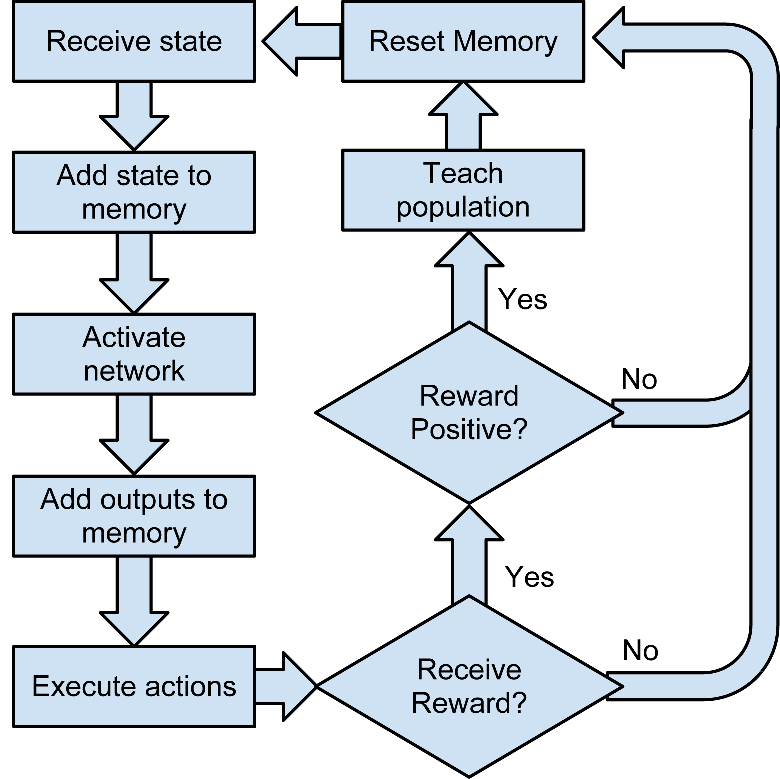
\includegraphics[scale=.6]{flowchart.pdf}
  \caption{Individuals remember their most recent inputs and the associated actions taken, and when rewarded will train other individuals on their recent actions.}
  \label{fig:flowchart}
\end{figure}


We use positive rewards to identify those actions on which we want to train agents.
As a result, it takes only the notion of a reward to allow our social learnng agents to begin to teach one another in real time.
 Previous approaches \cite{?} instead chose strong individuals as teachers and train weaker individuals on their actions.
By allowing any individual to train any other, we leverage a diversity of different behaviors in solving problems in a domain.

\section{Experimental Setup}
\label{sec:setup}
In this section we describe the experimental setup of our world.
We first describe the foraging somain, followed by the EA framework we use, NEAT.  Finally we outline the various experiments that we performed, and discuss what we varied and what we let remain constant in each.

    We use a foraging world in which agents move freely on a continuous toroidal surface which is 500 by 500 units.  
We populate our world with five types of plants - one with a strong reward, one with a weak reward, one which is neutral,one which deals a small penalty to an agent that eats it, and one that deals a large penalty.  
These plants are randomly distributed over the surface of the world.
  The domain is non-competitive and non-cooperative - each agent acts independently of all other agents.
  Each individual begins each generation in the center of the world, with a uniform orientation.
  The plants are randomly distributed around the world, and each individual has 1000 time steps in which to move and consume plants.
  Each plant has a radius of 5 units, and is eaten by any agent that comes within that radius and has not yet eaten the plant (each agent can only eat each plant once, and can only see plants it has not eaten.)
  
 The agents detect plants by means of sensors - they have 8 sensors for each plant, each of which covers 22.5 degrees, leading to a field of view of 180 degrees in front of them.
   They also have a sensor by which they can detect their current velocity.
   These sensors constitute the inputs to the neural network, and the individual's state.
Each agent has two effectors by which it can influence its position - one that controls $\delta v$, the change in velocity, and another that controls $\delta \theta$, the change in angle.
Each of these is one output node of a neural network.
  $\delta v$ is capped between -1 and 1 (the agents can speed up or slow down by one unit per timestep).
  $\delta \theta$ is capped between -30 and 30 degrees, the amount an agent can turn in a timestep.
  The maximum velocity of an agent is 5 units per timestep.
\subsection*{NEAT and SharpNEAT}
NEAT, the NeuroEvolution of Augmented Topologies algorithm for evolving neural networks, was the framework in which we performed our experiments.  
We used NEAT to generate a population of individuals to navigate the world.  
Each individual moving in the world is generated by a genome produced by NEAT, and the fitness of an individual is equal to the sum of all of the plants it eats in a generation (1000 timesteps).
NEAT then uses the fitnesses of these individuals to create new networks by modifying weights and adding and removing connections.

Because NEAT evolves recurrent neural networks, we used backpropagation through time to do our social learning \cite{somedude}. In Social Darwinian learning and Social Lamarkian learning, we backprop on other individuals whenever an individual receives reward. In Social Darwinism, as in Darwinan evolution in reality, the changes to the genome do not regress back to the phenome, and the offspring of an individual is determined by the phenome it had before it began learning.
In Social Lamarkism, the changes to the genome as the individual learns are propagated back to the phenome, and the offspring of an individual incorporate what that individual has learned in its lifetime into their phenomes.
\subsection*{Experiments} 
We ran several different experiments to investigate the effectiveness of our approach.
In each of these, we kept the size of the world stable at $500\times500$, and the population of agents constant at 100, with 10 different species.
We populated the world with 100 plants of varying reward such that the maximum reward is 3000 and the minimum reward is -3000.
All experiments were ran repeated in 30 independent trials and their results were averaged.

\section{Results}
\label{sec:results}
We next present the results of our three experiments that validate our non-hierarchical model. We begin by measuring the performance of social learning in both Darwinian and Lamarkian evolutionary paradigms. Following this, we determine whether social learning is effective when updates are performed only among the same species, with the goal of reducing the overall runtime cost of adding social learning. Finally, leverage the insights from the first two experiments and use Lamarkian social learning as a bootstrapping phase for Darwinian neuroevolution with no learning.

\begin{figure}
  \centering
    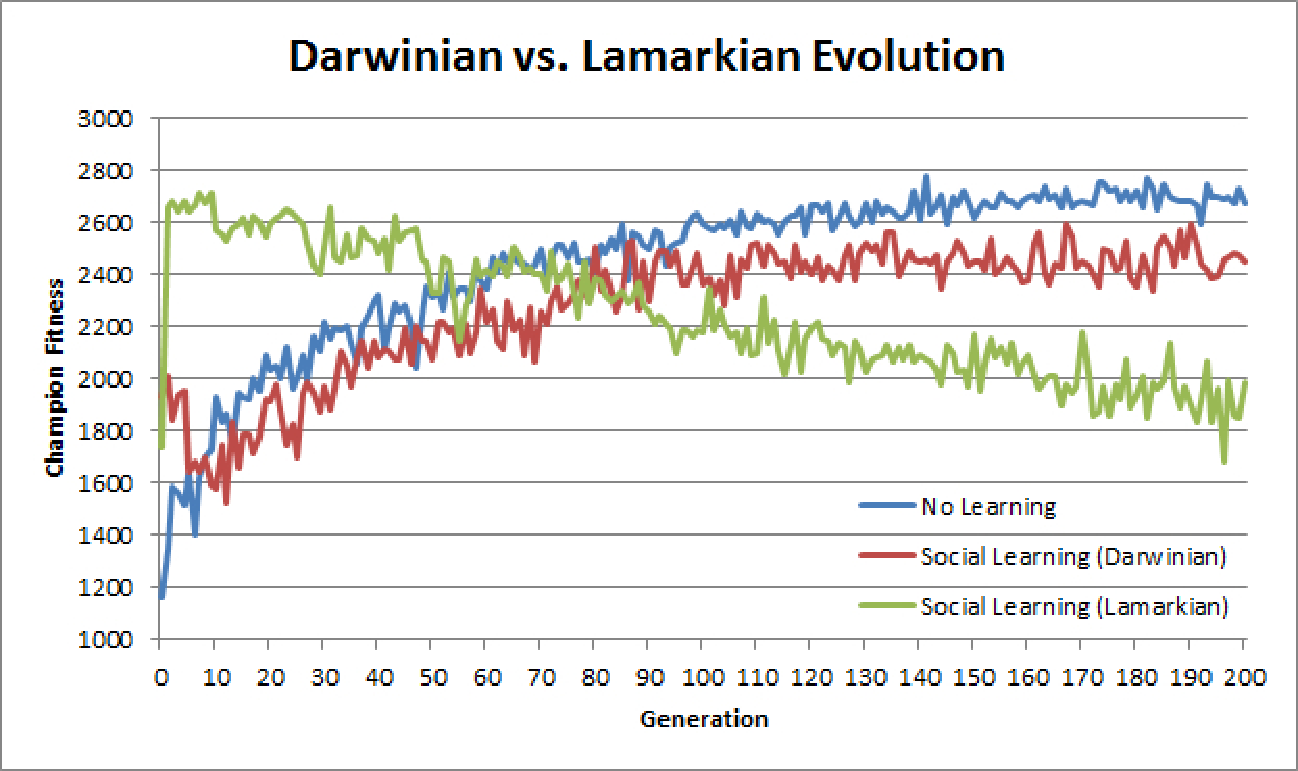
\includegraphics[scale=.35]{darwin_lamark.pdf}
  \caption{A comparison of the results for our non-hierarchical social learning algorithm in Darwinian and Lamarkian evolutionary paradigms.}
  \label{fig:darwin-lamark}
\end{figure}

\subsection*{Darwinian vs. Lamarkian}
Genetic inheritance paradigms in evolution falls into one of two main categories: Darwinian and Lamarkian. In Darwinian evolution, individual genomes are fixed and any knowledge gained or abilities gained during their lifetimes are not passed on to their offspring at birth. By contrast, in Lamarkian evolution an individual's genome changes as it learns throughout its life, and these changes are passed on to each of its offspring at birth. In the context of our experiments, this corresponds to whether the changes in each individual's neual network weights are propagated to their genome at the end of the generation.

Figure \ref{fig:darwin-lamark} shows the results of applying our non-hierarchical social learning algorithm to the foraging domain for both the Lamarkian and Darwinian paradigms. These results indicate that Lamarkian evolution is able to quickly reach a near-optimal score but then proceeds to degrade slowly over time. In the context of \textit{on-line} evolutionary learning algorithms, it has been shown \cite{whiteson2006evolutionary} that Darwinian evolution is preferrable to Lamarkian evolution in dynamic environments where adaptation is essential and the Baldwin effect \cite{simpson1953baldwin} may be advantagous. As adaptation is not necessary for our agents (i.e., the rewards of each plant type are the same in every generation), it is not exceedingly surprising that Lamarkian evolution outperforms Darwinian evolution initially.

However, the degradation of the Lamarkian fitness after generation 10 is surprising. We believe this is likely due to a ``regression to the mean'' effect where once the population reaches a sufficiently high fitness, the learning is derived more from the average individuals and less from the best individual. Thus, rather than the best individual pulling the other individuals' fitness up, the average individuals actually begin to pull the population as a whole down. A similar effect has been observed before \cite{denaro1996cultural}.

\begin{figure}
  \centering
    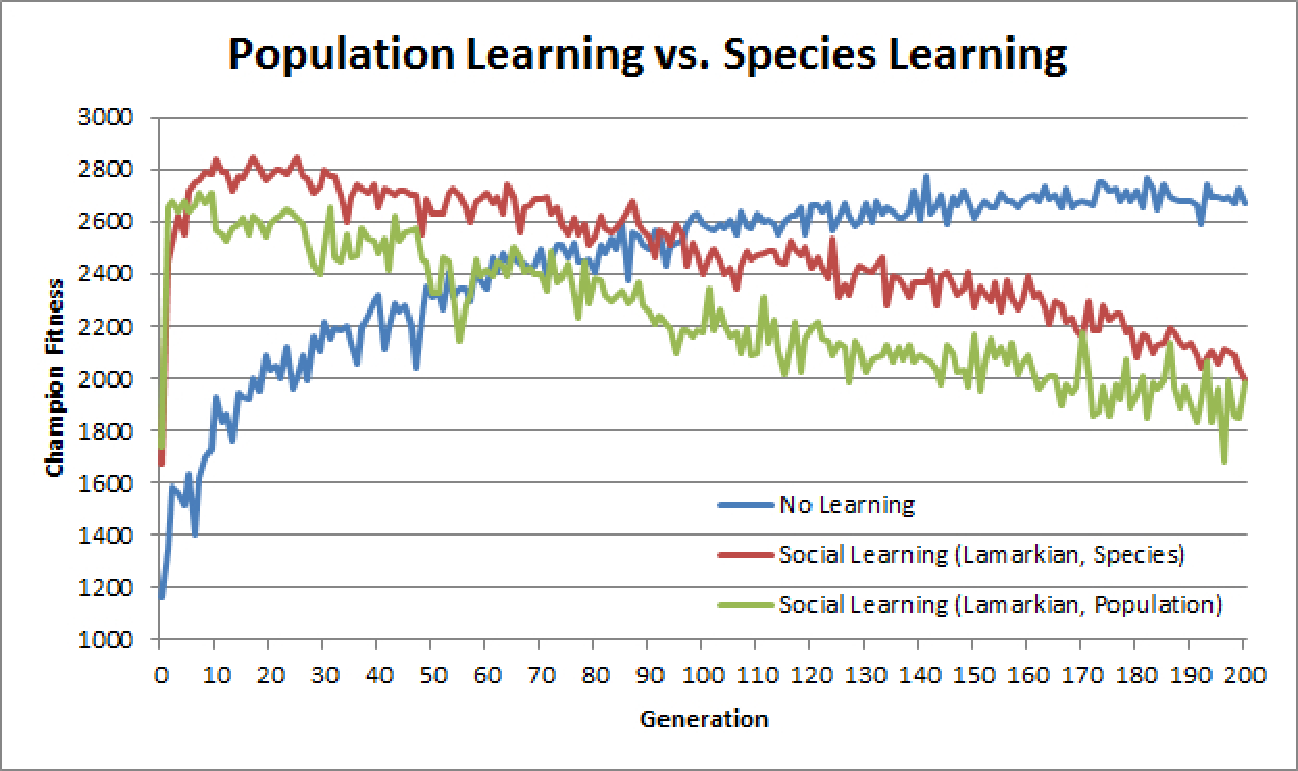
\includegraphics[scale=.35]{population_species.pdf}
  \caption{The results of agents learning from observations of the entire population compared to only agents in the same species.}
  \label{fig:population-species}
\end{figure}

\subsection*{Population vs. Species Learning}
While Lamarkian social learning is clearly able to find results quickly, it suffers from two main issues. As discussed above, the population begins to regress towards the mean after reaching the initial peak fitness. Also, while in many environments the simulation time required for running thousands of backprop on each individual may be irrelevant, to maximize practical efficiency it is important that our algorithm minimizes its overall impact on total runtime. To address these issues, we next consider a cultural variant of our social learning approach in which individuals only learn from observations of other individuals in the species. In practice, this significantly speeds up the application as it performs an order of magnitude less work for a population of 100 agents divided into 10 species.

Figure \ref{fig:population-species} shows the results comparing population-based and species-based social learning. Interestingly, the species-based social learning not only reaches a higher peak than the population-based method, but is also able to sustain its level of fitness for longer. Unfortunately, both approaches still suffer from the degradation of fitness characteristic of Lamarkian social evolution.

\begin{figure}
  \centering
    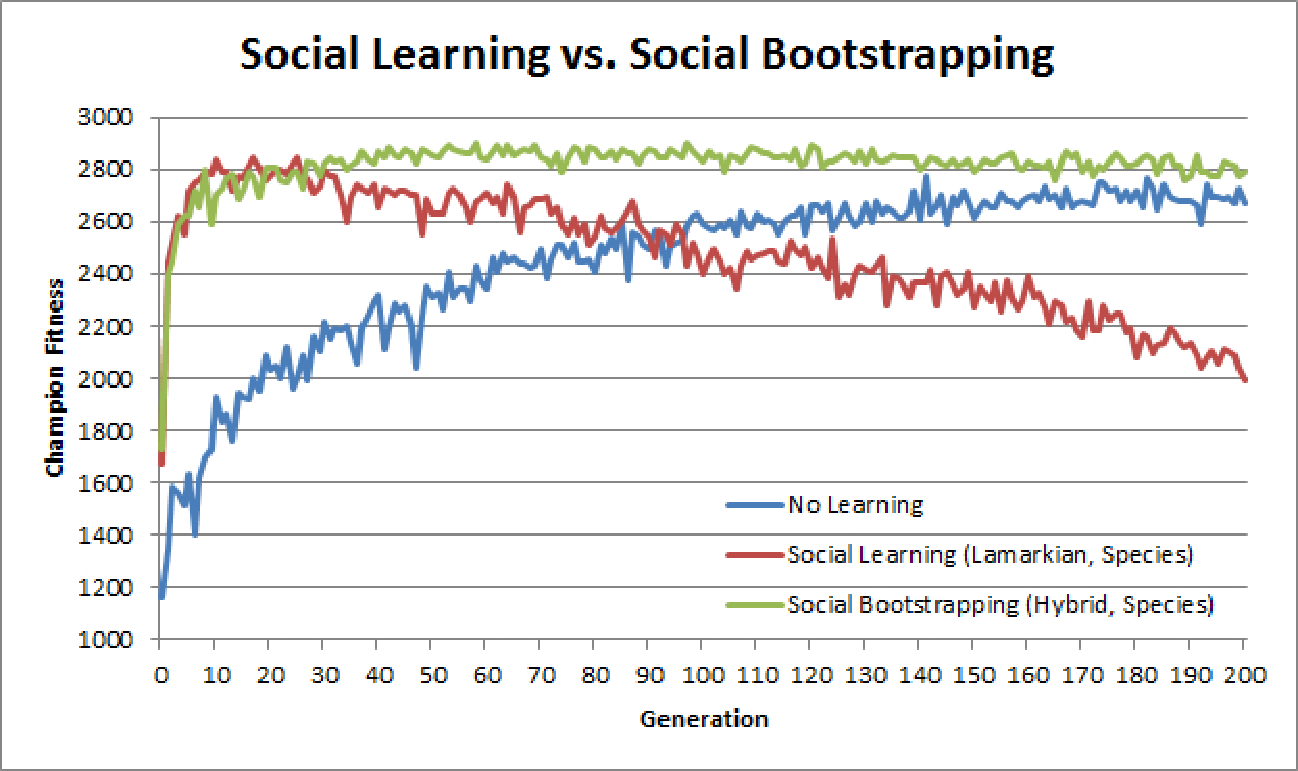
\includegraphics[scale=.35]{learning_bootstrapping.pdf}
  \caption{The results of our hybrid algorithm that uses social Lamarkian evolution to bootstrap the population for five generations then switches to traditional non-social Darwinian evolution.}
  \label{fig:learning-bootstrapping}
\end{figure}

\subsection*{Bootstrapping}
The ability to find a near-optimal fitness combined with the subsequent degradation of individuals in later generations suggests that social Lamarkian evolution may be best applied only in the initial generations. Figure \ref{fig:learning-bootstrapping} presents the results of a hybrid approach that uses social Lamarkian evolution for the first five generations to bootstrap the population, then transitions to the tradition non-social Darwinian evolution. The hybrid version is able to achieve a slightly higher (though not statistically significant) fitness than either comparison method and does not suffer from the degradation present in the pure social Lamarkian setup.

In the next section we present a brief discussion of related work on social learning in EAs.

\section{Related Work}
\label{sec:related}
Enhancing EAs with social and cultural learning is a flourishing area of research with a long and successful track record.
We next highlight relevant prior work and explain how our approach differs from previous efforts.

Cultural algorithms \cite{reynolds1994introduction} have been used frequently in Particle Swarm Optimization (PSO) \cite{kennedy1995particle}. Cultural algorithms maintain a ``belief space'' representing different categories of knowlege that the population has learned. New individuals are trained using this belief space in a student/teacher mode. In contrast, our agents maintain no separate repository of formal knowledge, but rather they learn from observations of others during their lifetime.

The ability of social learning to improve agents in a foraging domain is a popular setting that has explored by several researchers in recent years. Denaro et. al. \cite{denaro1996cultural} used a student/teacher model of cultural evolution without genetic inheritance and demonstrated that the population will continue to improve if Gaussian noise is added to the training examples. The NEW TIES system \cite{haasdijk2008social, vogt2010modeling} simulates a steady state evolution of decision tree agents where at each step the teacher agents probabilistically transmit their decisions and students probabilistically incorporate this knowledge. Acerbi et. al. \cite{acerbi2007social} use social learning to train embodied agents to mimic the behaviors of more experienced agents. Finally, de Oca et. al. \cite{de2011incremental} propose a methodology for incremental social learning in PSO to update Q-learning \cite{watkins1992q} value functions by randomly selecting two individuals from the population and combining their values for a given update. While all of these works are closely related and motivated by similar biological processes as our approach, they fundamentally all rely on the concept of students and teachers, and perform either no filtering or a reward-agnostic filtering of state-action pairs to be used in updating the population.

\section{Future Work}
\label{sec:future}

In this section we discuss potential future work that could be done to exploit non-hierarchical social learning and improve it as both a model of artificial life and a machine learning algorithm.
The most obvious extension to this work of social learning is to make it more social - to allow the agents to see and interact with one another.
To that end, evolving communication between agents is an important step in developing these ideas. 
Additionally, exploring the interactions between predators and social learning agents would be interesting future work. Despite being much weaker than many predators, humans thrive - perhaps because of our social brains.
Fundamentally, our work is related to Q-learning - comparing Q-learning with social learning is another avenue of future research.
%Reward-proportional updating

%Comparison to student/teacher models

%Dynamic domains

%Language (repellants and attractants, howler monkeys)

%Predators (co-evolution, fat agents)

%Q-Learning comparison (Ability gained per step)

%Variable length trajectories (Memory)

\section{Conclusions}
\label{sec:conclusions}
Summary
Hopeful and uplifting ending

%
% The following two commands are all you need in the
% initial runs of your .tex file to
% produce the bibliography for the citations in your paper.
\bibliographystyle{abbrv}
\bibliography{sigproc}  % sigproc.bib is the name of the Bibliography in this case
% You must have a proper ".bib" file
%  and remember to run:
% latex bibtex latex latex
% to resolve all references
%
% ACM needs 'a single self-contained file'!
%
%APPENDICES are optional
%\balancecolumns
%\appendix
%Appendix A
%\section{Headings in Appendices}
%The rules about hierarchical headings discussed above for
%the body of the article are different in the appendices.
%In the \textbf{appendix} environment, the command
%\textbf{section} is used to
%indicate the start of each Appendix, with alphabetic order
%designation (i.e. the first is A, the second B, etc.) and
%a title (if you include one).  So, if you need
%hierarchical structure
%\textit{within} an Appendix, start with \textbf{subsection} as the
%highest level. Here is an outline of the body of this
%document in Appendix-appropriate form:
%\subsection{Introduction}
%\subsection{The Body of the Paper}
%\subsubsection{Type Changes and  Special Characters}
%\subsubsection{Math Equations}
%\paragraph{Inline (In-text) Equations}
%\paragraph{Display Equations}
%\subsubsection{Citations}
%\subsubsection{Tables}
%\subsubsection{Figures}
%\subsubsection{Theorem-like Constructs}
%\subsubsection*{A Caveat for the \TeX\ Expert}
%\subsection{Conclusions}
%\subsection{Acknowledgments}
%\subsection{Additional Authors}
%This section is inserted by \LaTeX; you do not insert it.
%You just add the names and information in the
%\texttt{{\char'134}additionalauthors} command at the start
%of the document.
%\subsection{References}
%Generated by bibtex from your ~.bib file.  Run latex,
%then bibtex, then latex twice (to resolve references)
%to create the ~.bbl file.  Insert that ~.bbl file into
%the .tex source file and comment out
%the command \texttt{{\char'134}thebibliography}.
%% This next section command marks the start of
%% Appendix B, and does not continue the present hierarchy
%\section{More Help for the Hardy}
%The acm\_proc\_article-sp document class file itself is chock-full of succinct
%and helpful comments.  If you consider yourself a moderately
%experienced to expert user of \LaTeX, you may find reading
%it useful but please remember not to change it.
%\balancecolumns
% That's all folks!
\end{document}
